\subsection{\textit{Encoders} Rotativos Incrementais}
% Referencias:
% https://www.roboticsbusinessreview.com/news/differences-between-encoder-resolution-accuracy-and-precision/
% https://www.newtoncbraga.com.br/index.php/como-funciona/5454-mec128
% [Speed Measumment Using Rotary Encoders for High Performance ac Drives]
% [Speed Measurement Algorithms for Low-Resolution Incremental Encoder Equipped Drives: a Comparative Analysis]
% [A Simple Speed Feedback System for Low Speed DC Motor Control in Robotic Applications]
% [An Embedded System for Position and Speed Measurement Adopting Incremental Encoders]

% FALAR SOBRE O FUNCIONAMENTO BASICO
% CITAR OS DIFERENTES TIPOS
% FALAR DO GRAY CODE
% FALAR DO ERRO DE QUANTIZAÇÃO
Nessa seção será explicado um pouco dos principais conceitos envolvendo os \emph{Encoders} rotativos incrementais. Esse tipo de sensor é caracterizado por gerar um par de sinais defasados em $90^\circ$ a medida que o movimento rotacional é realizado.


Para o cálculo do módulo da velocidade de rotação do eixo do motor faz-se:
\begin{equation}
    |\omega_{medido}| = \frac{2\pi}{NPR}\frac{1}{\Delta{t}}
    \label{eq:modulo_omega_medido}
\end{equation}

Onde $NPR$ é o número pulsos por revolução em um canal. Já o intervalo $\Delta{t}$ é o intervalo entre bordas iguais em um canal, a Figura \ref{fig:sinal_em_quadratura_delta_t} ilustra esse intervalo para as bordas de subida de ambos os canais.\\

\begin{figure}[H]
    \centering
    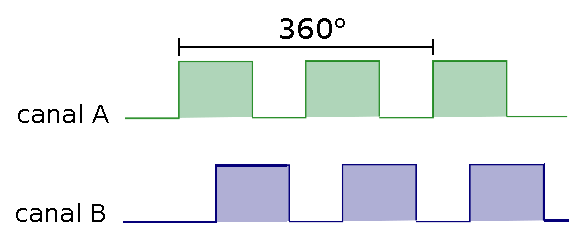
\includegraphics[width=0.5\textwidth]{imagens/ilustracoes/sinal_enquadratura_uma_revolucao.eps}
    \caption{Ilustração do sinal em quadratura em uma revolução completa do eixo do motor no sentido horário.}
    \label{fig:ilustracao_uma_revolucao}
\end{figure}

\begin{figure}[H]
    \centering
    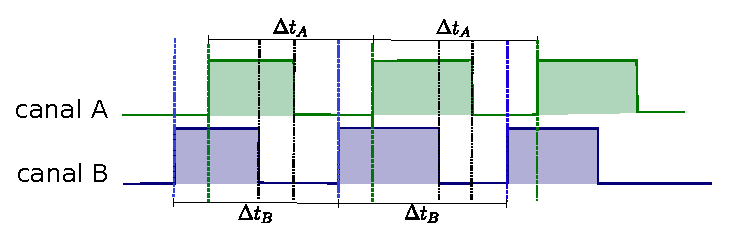
\includegraphics[width=0.6\textwidth]{imagens/ilustracoes/sinal_em_quadratura_sentido_CCW_detalhada.eps}
    \caption{Ilustração de um sinal em quadratura para uma revolução do eixo do motor sentido anti-horário para um \emph{Encoder} com a resolução de três pulsos por revolução, com destaque para o intervalo de tempo entre as bordas de subida de um mesmo canal.}
    \label{fig:sinal_em_quadratura_delta_t}
\end{figure}

% Please add the following required packages to your document preamble:
% \usepackage{graphicx}
\begin{table}[H]
\centering
\resizebox{0.5\textwidth}{!}{%
\begin{tabular}{cc|cc}
\multicolumn{2}{c|}{\textbf{\begin{tabular}[c]{@{}c@{}}Sentido\\     Horário\end{tabular}}} &
  \multicolumn{2}{c}{\textbf{\begin{tabular}[c]{@{}c@{}}Sentido\\ Anti-Horário\end{tabular}}} \\ \hline
\textbf{A} & \textbf{B} & \textbf{A} & \textbf{B} \\
1          & 0          & 1          & 0          \\
0          & 1          & 0          & 1         
\end{tabular}%
}
\caption{Código de 2 bits para identificar o sentido de rotação.}
\label{tab:tabela_simple_code}
\end{table}

Já para se obter o sentido de rotação do motor, faz-se uso do padrão \emph{Gray Code} gerado pela diferença de fase entre os diferentes canais de um mesmo sensor, uma maneira de fazer isso é ler os \emph{GPIO}'s associados aos canais do \emph{Encoder} e verificar o padrão em binário e inferir o sentido de rotação, a Figura \ref{fig:cw_signal} ilustrado isso para uma rotação no sentido horário e a Figura \ref{fig:ccw_signal} o anti-horário, esses códigos são apresentados na Tabela \ref{tab:tabela_simple_code}. Porém esse procedimento é pouco eficiente em medias e altas rotações, devido a alta taxa de erro na inferência do sentido.\\

Uma abordagem mais eficiente é armazenar os dois \emph{bits}(sendo canal A bit mais significado) e concatenar/somar com os últimos dois \emph{bits} (da leitura anterior) deslocados em dois (equivalente à multiplicar por $2^2$ ou operar bit-a-bit: $bits_{anteriores} \ll 2$), criando assim um padrão com $4$ \emph{bits}, sendo os dois mais significados o padrão da leitura anterior e os dois menos significativos a leitura atual. Esse procedimento é ilustrado para uma rotação no sentido horário e no sentido anti-horário respectivamente nas Tabelas \ref{tab:tabela_gray_code_cw} e \ref{tab:tabela_gray_code_ccw}, dessa forma gera-se quatro($4$) padrões/códigos que caracterizam um tipo de rotação.

\begin{figure}[H]
    \centering
    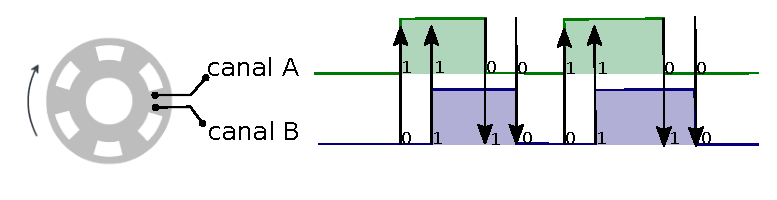
\includegraphics[width=0.7\textwidth]{imagens/ilustracoes/sinal_enquadratura_sentido_CW.eps}
    \caption{Sinal em quadratura para rotação no sentido horário.}
    \label{fig:cw_signal}
\end{figure}

% Please add the following required packages to your document preamble:
% \usepackage{graphicx}
\begin{table}[H]
\centering
\resizebox{0.5\textwidth}{!}{%
\begin{tabular}{c|c|c|c|c}
\textbf{$A_{ant}$} & \textbf{$B_{ant}$} & \textbf{$A_{atual}$} & \textbf{$B_{atual}$} & \textbf{DEC} \\ \hline
0 & 0 & 1 & 0 & 2 \\
1 & 0 & 1 & 1 & 11 \\
1 & 1 & 0 & 1 & 13 \\
0 & 1 & 0 & 0 & 4
\end{tabular}%
}
\caption{Gray Code para a rotação no sentido horário.}
\label{tab:tabela_gray_code_cw}
\end{table}

\begin{figure}[H]
    \centering
    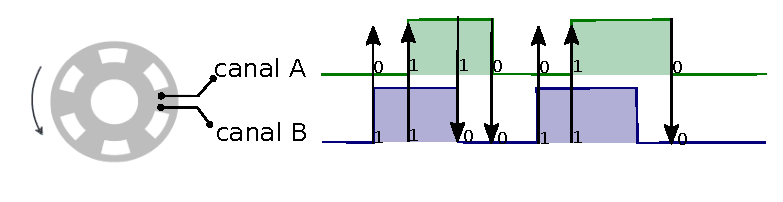
\includegraphics[width=0.7\textwidth]{imagens/ilustracoes/sinal_enquadratura_sentido_CCW.eps}
    \caption{Sinal em quadratura para rotação no sentido anti-horário.}
    \label{fig:ccw_signal}
\end{figure}

% Please add the following required packages to your document preamble:
% \usepackage{graphicx}
\begin{table}[H]
\centering
\resizebox{0.5\textwidth}{!}{%
\begin{tabular}{c|c|c|c|c}
\textbf{$A_{ant}$} & \textbf{$B_{ant}$} & \textbf{$A_{atual}$} & \textbf{$B_{atual}$} & \textbf{DEC} \\ \hline
0 & 0 & 0 & 1 & 1  \\
0 & 1 & 1 & 1 & 7  \\
1 & 1 & 1 & 0 & 14 \\
1 & 0 & 0 & 0 & 8 
\end{tabular}%
}
\caption{Codificação de 4 \emph{bits} para a rotação no sentido anti-horário.}
\label{tab:tabela_gray_code_ccw}
\end{table}


\begin{figure}[H]
    \centering
    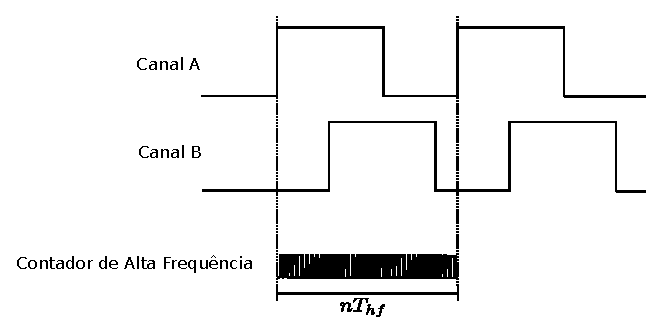
\includegraphics[width=\textwidth]{imagens/ilustracoes/ilustracao_medicao_encoder_por_periodo.eps}
    \caption{Ilustração de leitura de \emph{Encoder} periódica.}
    % \label{fig:my_label}
\end{figure}

% Speed Measumment Using Rotary Encoders
% for High Performance ac Drives
\begin{comment}
The output signals of an incremental encoder are usually two square waves with an electrical gap of 90'. The phase shift sign into these signals allows us to know the direction of rotation. It is also easy to quadruple the number of pulses per revolution (PPR), by detecting the edges of the encoder signals, as we can see in the Figure 1.

In order to achieve a high performance control system, it would be desirable to have an encoder with as many PPR as possible. Nevertheless, this will be limited by the higher rotor speed, due to the maximum frequency of the encoder electronics, just as by constructive limitations, mainly in the radial grating.

There are two basic ways to get the rotor speed by means of an encoder: counting the encoder pulses for a known time, what is a frequencimeter. or measuring the width of a pulse, wath is a periodimeter. We will discuss the advantages and disadvantages of both methods, along with some practical considerations.

SPEED MEASUREMENT USING A FREQUENCIMETER

The simplest way to get the rotor speed is counting the number of pulses from the encoder p, for a fixed time ,T, which is the speed (torque) loop period (Figure 1). Being a the corresponding angle of each encoder pulse, the rotated angle in a period will be:

\begin{equation}
    \alpha_{total} = n \alpha
\end{equation}

therefore the rotor speed will be

\begin{equation}
    \omega_{rotor} = \frac{\alpha_{total}}{T}
\end{equation}

The main disadvantage of this method is that, in each period, the measured angle a, will be always an integer multiple of a, which produces a quantization error in the estimated speed, with a maximum value of $\alpha_{total}/T$.

Obviously, this error will decrease as a decreases, that is, as the number PPR increases, and as the period T increases

We can conclude that a frequencimeter shows quantization problems, which makes them not very suitable at lower speeds. These could be solved by using digital filters, or increasing the period of the torque controller (which at last is a kind of moving average filter). Nevertheless, both solutions introduce a delay obtaining the velocity, which can degrade the control system perfotman~e

SPEED MEASUREMENT USING A PERIODIMETER

If we use a periodimeter, we will get the speed not by counting pulses from the encoder, but by counting a high frequency (HF) clock

Let $\alpha_p$ be the corresponding angle to the higher part of an encoder pulse (half of its period), t the period of the HF clock, and n the number of HF pulses arrived at the HF counter. Then, the time spent on an encoder pulse, $T_e$ is:

\begin{equation}
    T_e = n t
\end{equation}

Rotor speed can be obtained as:

\begin{equation}
    \omega_{rotor} = \frac{\alpha_p}{T_e}
\end{equation}

As with the frequencimeter, here also there is a quantization error because of the time T,, which will be always an integer multiple of t With a fixed HFclock frequency, this error will increase as n decreases, that is, as the encoder rotates faster, but it provides accurate measurements at lower speeds. Because the variable with quantization noise is now in the denominator, its effects are much more important than in the frequencimeter.

An additional advantage at low speed is that, as it only needs one pulse to get the speed, the delay is minimal, which is very important at lower speeds.

It also possible to use quadruple frequency. Of course, this reduces the precision, and therefore the maximum velocity where this method is suitable, but also, and this is much more important, it reduces the delay obtaining the velocity when the motor works at low speed. Nevertheless, this method produces stability problems in the zero speed cross. Figure 8 shows an inversion with two possible situations in the encoder output signals. Supposing that there is no quadruple frecuency, and PHASE A controls the HF counter, we see that at the encoder pulse end, the counter has a wrong value, because about half of the HF pulses arrived on each direction of rotation.

The accuracy of the periodimeter is, more than the frequencimeter, related to the accuracy of the encoder, which in general depends on the errors in the radial grating, and the eccentricity of the graduated disk to the bearing.

% Speed Measurement Algorithms for
% Low-Resolution Incremental Encoder Equipped
% Drives: a Comparative Analysis

A. Frequency measurement

The classical and probably the simplest method to measure rotor speed is the direct measure of the frequency of the encoder pulses. Typically the number of the observed pulses inside a given and constant-width time-window is counted. Angular speed is then approximated to the discrete incremental ratio, that is constant speed is considered inside the observation windows:

\begin{equation}
    \omega = \frac{d\theta}{dt} \cong \frac{\Delta{\theta}}{T_{sc}} \cong \frac{2 \pi \Delta{N}}{N_{p}T_{sc}}[rad.s^{-1}] \xrightarrow{} \frac{60 \Delta{N}}{N_{p}T_{sc}} [RPM]
\end{equation}

where N p is the number of pulses per revolution (after quadrature decoding), T sc is the time-window and ∆N is the number of observed pulses inside that window. As a result, one has a quantisation error superimposed to the effective mean speed inside the observation window which depends on the uncertainty on the measured number of pulses ∆N, caused by the lack of synchronisation between encoder pulses and the observation window itself.

The speed measurement quantisation error $\Delta{\omega}$ is:

\begin{equation}
    \Delta{\omega} = \frac{2\pi}{N_{p}T_{sc}}[rad.s^{-1}] \xrightarrow{} \frac{60}{N_{p}T_{sc}}[RPM]
\end{equation}

Equation (2) shows that the quantisation error is independent from the operating speed and it depends only on the number of encoder pulses per revolution and the observation time window. Therefore the relative accuracy of the method is a function of the speed itself, as expressed by the following formula:

\begin{equation}
    e_{\omega}\% = \frac{2\pi}{\omega N_{p} T_{sc}}.100
\end{equation}

\begin{figure}[H]
    \centering
    
\includegraphics[width=\textwidth]{imagens/ilustracoes/ilustracao_erro_de_quantizacao.eps}
    \caption{Ilustração do erro de quantização na medição de velocidade de rotação.}
    \label{fig:ilustracao_erro_quantizacao}
\end{figure}


A commonly adopted way to reduce quantisation error, especially in the low speed region, is to increase the speed sampling time and control period, but this solution reduces the bandwidth of the controller. Low-pass filtering can be adopted aiming at reducing steady-state as well as transient error and remove the excess quantisation error, but the additional lag time introduced by the filter degrade the performance of the speed control loop and sometimes is not tolerable. Good results are achieved by employing moving average based filtering. The width of the window buffer has to be chosen considering the required accuracy of steady-state measurement error and the dynamical performance degradation of the drive. Gain of accuracy is therefore proportional to the length of the window buffer used for filtering.

The implementation of the frequency measuring method is very straightforward, as it requires only the computation of ∆N and one multiplication for the constant terms in (1) if the basic measurement is considered. Incremental position measurement is almost always performed by dedicated quadrature decoder hardware, commonly found inside dedicated microcontrollers.

B. Period measurement

An alternative solution to the reduction of the measurement error is to switch from frequency to period measurement at a certain level of (low) speed. The measurement is realised by counting the number of periods of a high frequency signal inside one (or more) encoder pulses, Fig. 3. The following formula is obtained under the hypotesis that motor speed is constant and only one period of the encoder signal is considered:

\begin{equation}
    \omega = \frac{d\theta}{dt} \cong \frac{\Delta{\theta}}{nT_{hf}} \cong \frac{2\pi}{N_{p} n T_{hf}} [rad.s^{-1}] \xrightarrow{} \frac{60}{N_{p} n T_{hf}} [RPM]
\end{equation}

A speed sample can be calculated each period of the encoder signals. Speed sampling period is thus a function of motor speed:

\begin{equation}
    T_{\omega}(\omega) = \frac{2\pi}{N_{p}\omega} [s]
\end{equation}

The accuracy of the measurement is related to the ratio between the period of the high frequency counter and that of the encoder signals, that is not an integer value as it depends on motor speed. A calculation of absolute and percentage errors is extremely difficult as it involves non-linear rounding functions. A worst-case condition error could be calculated instead by considering the absolute error of one high frequency pulse, leading to a maximum percentage error limiting locus given by the following formula, i.e. roughly linear with speed:

\begin{equation}
    e_{\omega}\% = \frac{T_{hf}}{ \frac{2\pi}{N_{p} \omega} - T_{hf} }.100 \cong \frac{\omega N_{p} T_{hf}}{2\pi}
\end{equation}

At very low speed the number of high frequency pulses can be extremely high and saturation of the digital timer employed for measurement can occur. Also a speed sample is not available each speed control period, needing an adaptation of the control parameters. In that situation, the quadrature decoding of the encoder pulses can be exploited in order to reduce the width of the measuring window by a factor of four or a reduction of the frequency of the timer can be considered.

The former solution allows to reduce the speed sampling period and improve the control performance of the drive, but makes the measuring system more sensitive to sensor nonidealities, including variations in the transition locations from their nominal values and phasing errors between encoder channels. When low-cost and low-resolution sensors are employed, nonidealities play the major role in the determination of period measuring errors and has to be carefully analysed in drive design phase. The latter solution needs to switch on-line the frequency of the timer and adapt the coeffients of the equations above.

The implementation of the period measuring method is also straightforward as it requires a simple timer capture unit, commonly found inside recent microcontrollers.

% A Simple Speed Feedback System for Low Speed
% DC Motor Control in Robotic Applications

The relationship between the measured frequency using PIC microcontroller and the percentage error is shown in Fig. 2. The percentage error is given as:

\begin{equation}
    e\% = \frac{F_m - F_a}{F_a}.100
\end{equation}

where F m and F a denote the measured and actual frequencies. It is observed that as the frequency increases, the error in the frequency measured from PIC increases linearly, that is, there is a linear relationship between error and frequency.

\end{comment}